\documentclass[11pt]{article}

\usepackage{pablo}
\usepackage{yhmath}
  \usetikzlibrary{3d,calc}

\usepackage[a5paper,margin=1.4cm]{geometry}

\pagestyle{empty}
\begin{document}

\begin{center}
  \textsc{DM}
  ---
  {
    \Large
    Géométrie dans l'espace

    \hrule
  }
\end{center}

\begin{em}
  À rendre le mardi 18 mars.
\end{em}

\begin{exercice}[Perspective cavalière]
  On considère le triangle suivant, avec les longueurs $BC=13cm$, $AC=15cm$, $AH=3cm$.

  \begin{tikzpicture}[scale=0.5]
    \draw (0,0) node[left]{$A$}-- (3,5) node[above]{$B$} -- (15,0) node[right]{$C$} -- cycle;
    \draw (3,0) node[below]{$H$} -- (3,5) node[midway,right]{$I$} node[midway]{-};
    \draw (3,0.5) -- ++(0.5,0) -- ++(0,-0.5);
  \end{tikzpicture}

  \begin{enumerate}
    \item Montrer que $BH=5cm$.
    \item Dessiner en perspective cavalière la pyramide de base $ABC$, de hauteur $7cm$, le sommet de la pyramide étant à la verticale du point $I$ milieu de $BH$. On prendra 30\up{o} comme angle des fuyantes, et 0,8 comme coefficient de réduction.
  \end{enumerate}
\end{exercice}

\hfill\emph{Tourner la page.}
\newpage

\begin{exercice}[Surface d'un cône]~

  \begin{center}
    \hspace{\stretch{1}}
  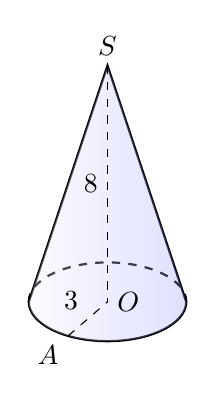
\begin{tikzpicture}
    \draw[thick] (-1,0) arc (180:360:1cm and 0.5cm) -- (0,3) -- cycle;
    \draw[thick,dashed] (-1,0) arc (180:0:1cm and 0.5cm);
    \shade[thick,left color=blue!5!white,right color=blue!40!white,opacity=0.3] (-1,0) arc (180:360:1cm and 0.5cm) -- (0,3) -- cycle;
    \draw[dashed] (240:1cm and 0.5cm) -- (0,0) node[midway,above left]{$3$};
    \draw[dashed] (0,3) -- (0,0) node[midway,left]{$8$};
    \draw (0,0) node[right]{$O$};
    \draw (0,3) node[above]{$S$};
    \draw (240:1cm and 0.5cm) node[below left]{$A$};
  \end{tikzpicture}
    \hspace{\stretch{1}}
  \begin{tikzpicture}[scale=0.3]
    \draw (0,0) circle (3);
    \draw (0,{3+sqrt(73)}) node[above]{$O$} -- ++({-sqrt(73)*sin((1080/sqrt(73))/2)},{-sqrt(73)*cos((1080/sqrt(73))/2)}) node[left]{$B$} arc ({(540-(1080/sqrt(73)))/2}:{(540+(1080/sqrt(73)))/2}:{sqrt(73)}) node[right]{$C$}-- cycle;
    \draw[draw=none] (0,{3+sqrt(73)}) -- ++({-sqrt(73)*sin((1080/sqrt(73))/2)},{-sqrt(73)*cos((1080/sqrt(73))/2)}) node[midway,above]{$R$};
    \draw[dashed] (0,0) -- ++(33:3) node[midway,below]{$3$};
    \draw ({-2*sin((1080/sqrt(73))/2)},{3+sqrt(73)-2*cos((1080/sqrt(73))/2)}) arc ({(540-(1080/sqrt(73)))/2}:{(540+(1080/sqrt(73)))/2}:{2});
    \draw (0,{3+sqrt(73)-2}) node[below]{$\alpha$};
  \end{tikzpicture}
    \hspace{\stretch{1}}
    ~
  \end{center}

  On considère un cône de révolution, dont la base est un cercle de rayon 3~cm, et de hauteur 8~cm. Le but de l'exercice est de déterminer l'aire de ce solide, dont le patron est donné à droite.

  Dans la suite de l'exercice, toutes les longueurs considérées sont en centimètres.

  \begin{enumerate}
    \item On considère le triangle $OAS$. Quelle est sa nature ? Lire sur le dessin les longueurs des segments $[AO]$ et $[OS]$ ? En déduire que $SA=\sqrt{73}$.
  \end{enumerate}
  La longueur notée $R$ sur le patron étant égale à $SA$, nous avons montré que $R=\sqrt{73}$. Nous allons maintenant calculer la valeur de l'angle $\alpha$.
  \begin{enumerate}
      \setcounter{enumi}{1}
    \item Calculer le périmètre de la base.
    \item La longueur de l'arc de cercle $\wideparen{BC}$ est égale au périmètre de la base. D'autre part, le périmètre d'un arc de cercle est proportionnel à l'angle correspondant. Compléter le tableau de proportionnalité suivant.

      \begin{center}
      \begin{tabular}{p{10em}||c|c}
        Angle & $\alpha$ & 360 \\
        \hline
        Longueur de l'arc de cercle de rayon $\sqrt{73}$ & & \\
      \end{tabular}
    \end{center}
    \item En déduire que $\alpha=\frac{1080}{\sqrt{73}}$
    \item L'aire d'une section de disque étant proportionnelle à son angle, calculer l'aire de la section de disque $OBC$.
    \item En déduire l'aire du cône.
  \end{enumerate}
\end{exercice}

\newpage

\setcounter{exercice}{0}
\begin{center}
  \textsc{DM}
  ---
  {
    \Large
    Géométrie dans l'espace

    \hrule
  }
\end{center}

\begin{em}
  À rendre le mardi 18 mars.
\end{em}

\begin{exercice}[Perspective cavalière]
  On considère le triangle suivant, avec les longueurs $BC=13cm$, $AC=15cm$, $AH=3cm$.

  \begin{tikzpicture}[scale=0.5]
    \draw (0,0) node[left]{$A$}-- (3,5) node[above]{$B$} -- (15,0) node[right]{$C$} -- cycle;
    \draw (3,0) node[below]{$H$} -- (3,5) node[midway,right]{$I$} node[midway]{-};
    \draw (3,0.5) -- ++(0.5,0) -- ++(0,-0.5);
  \end{tikzpicture}

    Dessiner en perspective cavalière la pyramide de base $ABC$, de hauteur $7cm$, le sommet de la pyramide étant à la verticale du point $I$ milieu de $BH$. On prendra 30\up{o} comme angle des fuyantes, et 0,8 comme coefficient de réduction.
\end{exercice}

\hfill\emph{Tourner la page.}
\newpage

\begin{exercice}[Surface d'un cône]~

  \begin{center}
    \hspace{\stretch{1}}
  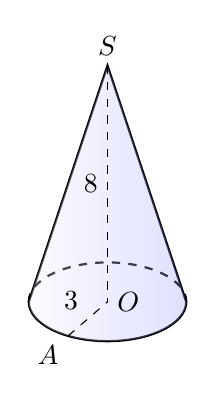
\begin{tikzpicture}
    \draw[thick] (-1,0) arc (180:360:1cm and 0.5cm) -- (0,3) -- cycle;
    \draw[thick,dashed] (-1,0) arc (180:0:1cm and 0.5cm);
    \shade[thick,left color=blue!5!white,right color=blue!40!white,opacity=0.3] (-1,0) arc (180:360:1cm and 0.5cm) -- (0,3) -- cycle;
    \draw[dashed] (240:1cm and 0.5cm) -- (0,0) node[midway,above left]{$3$};
    \draw[dashed] (0,3) -- (0,0) node[midway,left]{$8$};
    \draw (0,0) node[right]{$O$};
    \draw (0,3) node[above]{$S$};
    \draw (240:1cm and 0.5cm) node[below left]{$A$};
  \end{tikzpicture}
    \hspace{\stretch{1}}
  \begin{tikzpicture}[scale=0.3]
    \draw (0,0) circle (3);
    \draw (0,{3+sqrt(73)}) node[above]{$O$} -- ++({-sqrt(73)*sin((1080/sqrt(73))/2)},{-sqrt(73)*cos((1080/sqrt(73))/2)}) node[left]{$B$} arc ({(540-(1080/sqrt(73)))/2}:{(540+(1080/sqrt(73)))/2}:{sqrt(73)}) node[right]{$C$}-- cycle;
    \draw[draw=none] (0,{3+sqrt(73)}) -- ++({-sqrt(73)*sin((1080/sqrt(73))/2)},{-sqrt(73)*cos((1080/sqrt(73))/2)}) node[midway,above]{$R$};
    \draw[dashed] (0,0) -- ++(33:3) node[midway,below]{$3$};
    \draw ({-2*sin((1080/sqrt(73))/2)},{3+sqrt(73)-2*cos((1080/sqrt(73))/2)}) arc ({(540-(1080/sqrt(73)))/2}:{(540+(1080/sqrt(73)))/2}:{2});
    \draw (0,{3+sqrt(73)-2}) node[below]{$\alpha$};
  \end{tikzpicture}
    \hspace{\stretch{1}}
    ~
  \end{center}

  On considère un cône de révolution, dont la base est un cercle de rayon 3~cm, et de hauteur 8~cm. Le but de l'exercice est de déterminer l'aire de ce solide, dont le patron est donné à droite.

  Dans la suite de l'exercice, toutes les longueurs considérées sont en centimètres.

  \begin{enumerate}
    \item Montrer que $SA=\sqrt{73}$.
    \item Calculer le périmètre de la base.
    \item Le périmètre d'un arc de cercle étant proportionnel à l'angle correspondant, en vous servant du patron du cône, montrer que $\alpha=\frac{1080}{\sqrt{73}}$
    \item L'aire d'une section de disque étant proportionnelle à son angle, calculer l'aire de la section de disque $OBC$.
    \item En déduire l'aire du cône.
  \end{enumerate}
\end{exercice}

\end{document}
